% Chapter Template

\chapter{Explanation Maps Generation} % Main chapter title

\label{Chapter:Interpretation} % Change X to a consecutive number; for referencing this chapter elsewhere, use \ref{ChapterX}

In this chapter we present work done regarding the interpretation goal of the thesis. In medical diagnosis tasks it is important not only the accuracy of predictions but also the reasons behind decisions. Self-explainable models enable the physicians to contrast the information reported by the model with their own knowledge, increasing the probability of a good diagnostic, which may have a significant influence in patient's treatment.  The aim of this work is the elaboration of a general purpose interpretation algorithm, able to generate pixel maps that help in the interpretation of classification results reported by the model. With this model, it is possible to generate automatically very precise lesion maps that are learn indirectly only from general classification information. The model encodes statistical regularities present in data and the model presented in this chapter is able to visualize them. The system is organized using individual building blocks that make it easily transferable to be used with other architectures and in other completely different domains.

\section{Introduction}

Different attempts have been done for interpreting the results reported by neural networks. In \citep{zeiler2014visualizing} a network propagation technique is used for input-space feature visualization. After this work, \citep{bach2015pixel} used a pixel-wise decomposition for classification problems. This decomposition could be done in two ways: considering the network as a global function, disregarding its topology (functional approach) or using the natural properties of the inherent function topology for applying a message passing technique, propagating back into the pixel space the last layer output values. After this work, in \citep{montavon2017explaining} they used a so-named Deep Taylor decomposition technique to replace the inherently intractable standard Taylor decomposition, using a multitude of simpler analytically tractable Taylor decompositions.

In this chapter we follow an approach similar to pixel-wise decomposition taking into account the compositional nature of the topology, as in \citep{zeiler2014visualizing} and \citep{bach2015pixel}. The concept of \emph{score} in our chapter is similar to the concept of \emph{relevance} used in the layer-wise relevance propagation method. The novelty of our approach comes from the fact that we assume that there are two factors that contribute to output score: one is the input-space contribution, while the other is a contribution coming from the receptive fields of each layer. This last contribution depends solely on the parameters of each layer, thus being independent from the input-space. The second factor is not an attribute of the individual pixels that has to be propagated back, but a contribution of the receptive field (RF) that represents the layer as an individual entity. Therefore, we only propagate back the score part that depends on the precedent input in each layer. In the proposed explanation model, we consider the constant part as a property of the RF of each layer. This approach allows us to do an exact propagation of the scores using a de-convolutional approach. Differing also from \citep{zeiler2014visualizing}, our method allows the integration of batch normalization and of other typical neural network block constituents into the score propagation. A full set of score propagation blocks with the more typical DL functional constituents is derived in the chapter, in order to facilitate the portability of this new explanatory method to other networks and applications.

%This interpretation model is tested in our application research area: Diabetic Retinopathy. DR is a leading disabling chronic disease  and  one of the main causes of blindness and visual impairment in developed countries for diabetic patients. Studies reported that 90\% of the cases can be prevented through early detection and treatment. Eye screening through retinal images is used by physicians to detect the lesions related with this disease. Due to the increasing number of diabetic people, the amount of images to be manually analyzed is becoming unaffordable. Moreover, training new personnel for this type of image-based diagnosis is long, because it requires to acquire expertise by daily practice. Medical community establishes a standardized classification based on four severity stages \citep{diaclass} determined by the type and number of lesions (as micro-aneurysms, hemorrhages and exudates) present in the retina: class 0 referring to no apparent Retinopathy, class 1 as a Mild Non-Proliferative Diabetic Retinopathy (NPDR), class 2 as Moderate NPDR, class 3 as a Severe NPDR and class 4 as a Proliferative DR. 

%In this section we present a \emph{DR interpretable image classification model}
This interpretation model is tested in our application research area: Diabetic Retinopathy for grading the level of disease. This model is able to report the predicted class and also to score the importance of each pixel of the input image in the final classification decision. In such a way, it is possible to determine which pixels in the input image are more important in the final decision and facilitate the human experts an explanation to verify the results reported by the model.

\section{Related work}\label{score:sec:related}

In last years, different approximations have been proposed to convert the initial DL black box classifiers into \emph{interpretable classifiers}. In the next sections we introduce the most successful interpretation models existing today: sensitivity maps, layer-wise relevance propagation and Taylor decomposition models. 

\subsection{Sensitivity maps}

Sensitivity maps \citep{DBLP:journals/corr/SimonyanVZ13} are pixel-space matrices obtained from the calculation of $ \frac{\partial f(I)}{\partial I_{c,i,j}} \quad \forall c,i,j$, where $I$ is the input image and $f(I)$ is the DL function. These matrices are easy to calculate for deep neural networks because they use the same backpropagation rules that are used during training, requiring only one more backpropagation step for reaching the input-space. The problem with this approach is that there is no direct relationship between $f(I)$ and $\nabla f(I)$. The main concern of these models is that being the objective to explain $f(x)$, $ \frac{\partial f(I)}{\partial I_{c,i,j}}$ is only giving information about the local change of the function. For high non-linear functions, like deep neural networks, the local variation is pointing to the nearest local optimum, which should not necessarily be in the same direction that the global minimum \citep{baehrens2010explain}.


\subsection{Layer-wise relevance propagation} 

In \citep{bach2015pixel} the authors split the total score of a classification into individual \emph{relevance scores} $R_d$ that act as a positive or negative contributions to the final result. 

The method has the next general assumptions: the first one is the nature of the classification function, which has to be decomposable into several layers of computation (like a deep neural network), the second is about the fact that the total relevance must be preserved from one layer to another, which means that the relevance of one layer is equal to the ones of all other layers (eq. \ref{score:eq:relevance-conservation}) and, finally, the relevance of each node must be equal to the sum of all the incoming relevance messages of such node and also equal to the sum of all the outgoing relevance messages from the same node (eq. \ref{score:eq:relevance-message-value}).

\begin{equation}
f(x) = \sum_{d \in l+1}R_d^{(l+1)} = \sum_{d \in l}R_d^{(l)} = ... = \sum_{d}R_d^{(1)}
\label{score:eq:relevance-conservation}
\end{equation}

where $R_d^{(l)}$ is the relevance of node $d$ in layer $l$.

\begin{equation}
R_{i \leftarrow k}^{(l,l+1)} = R_k^{(l+1)} \frac{a_i \omega_{ik}}{\sum_{h} a_h \omega_{hk}}
\label{score:eq:relevance-message-value}
\end{equation}

where $R_{i \leftarrow k}^{(l,l+1)}$ is the relevance message passing from node $k$ located in layer $l+1$ to node $i$, located in layer $l$; $a_i$ is the activation of node $i$ and $\omega_{ij}$ is the weight connecting node $i$ and $j$.

\subsection{Taylor-type decomposition} 

Another way for solving the interpretability problem is using the classification function gradient to calculate the next Taylor approximation \citep{bach2015pixel}:

\begin{equation}
f(I) \approx f(I_0) + \nabla(I_0) [ I - I_0] = f(I_0) + \sum_{c=1}^C \sum_{i=1}^{H} \sum_{j=1}^W \frac{\partial f}{\partial I_{c,i,j}}(I_{c,i,j} - I_{0 c, i, j}) 
\label{score:eq:taylor}
\end{equation}

Being $I_0$ a free parameter that should be chosen in a way that $f(I_0) = 0$ in the case that $f(I)$ is defined as a function that reports a value greater than one when belongs to the class, and lower than 0 otherwise. Defined in such a way, $f(I) = 0$ express the case of maximum uncertainty about the image. Finding $I_0$ allows us to express $f(I)$ as:

\begin{equation}
f(I) \approx \nabla(I_0) [ I - I_0] = \sum_{c=1}^C \sum_{i=1}^{H} \sum_{j=1}^W \frac{\partial f}{\partial I_{c,i,j}}(I_{c,i,j} - I_{0 c, i, j}) \quad  being \quad f(I_0) = 0
\label{score:eq:relevance-approximation}
\end{equation}

Equation \ref{score:eq:relevance-approximation} is per se an explanation of $f(I)$ dependent only of the derivative function and of $I_0$. The main concern of this approach is finding a valid root that is close to the analyzed image $I$ using the Euclidean norm. In that way, we are approximating the function with a order 1 Taylor expansion and the residuum is proportional to the Euclidean distance between both points. Different ways for finding $I_0$ have been proposed. For example, doing a unsupervised search of $f(I)$ over the training set, looking for those images reporting $f(I)$ near 0 and averaging them for finding $I_0$.

\subsection{Deep Taylor decomposition}

Deep Taylor decomposition \citep{montavon2017explaining} uses an approximation that combines the layer-wise and Taylor type models. Taking advantage of the compositional nature of DL models, this approach assumes also the decomposability of the relevance function, considering the existence for every node of a partial relevance function $R_i(a_i)$ that depends on the activation. It considers this function unknown and applies a Taylor decomposition through a root point. Summing up all the individual contributions, using the relevance conservation property defined in the previous models, makes possible the propagation of intermediate relevance scores until eventually reach the input-space. Then, it generates a heat-map of the total relevance of the prediction in the input image. 

\section{Receptive field score distribution model} \label{score:sec:math}

In this section we explain the new method proposed in this thesis for distributing the output score into the previous layers in DL models \citep{de2017deep}. We hypothesize that the output score of a particular classification model is not only due to pixel score contributions but also due to all the contributions of the receptive fields analyzed by the network. In next sections we will prove that, for all typical neural network types of layers, the output score can be expressed as the sum of layer's constants plus a value proportional to the layer's input. Pixel-wise explanation model uses a similar approach for propagating backwards the scores, but with an important difference: pixel-wise \citep{bach2015pixel} propagates back not only the input layer contribution, but also constants,such as the bias, etc. Such a way of propagating backwards the scores breaks the linear transformation. A way of maintaining the linear transformation is propagating backwards only the part that depends on the input, leaving the other part as a contribution of the layer (ie. of the receptive field). As the biases are not propagated, the normalization term used in pixel-wise method is not required anymore. Although neural network design is non-linear, score back-propagation is linear over the activated nodes. Nonlinear phase takes place in the forward pass, but the backward part only takes place over the activated nodes. In our formulation, we consider the score entering into a node as the combination of two parts: one that can be transformed into a linear function dependent on the activated inputs and another one that is constant for the considered node. Then, the final score is expressed as the sum of contributions of all nodes belonging to the studied feature space (or pixel space) plus a constant score for the contribution of each node to every following layer.
Such node constant scores depend on layer parameters and, in some way, on the output activations of the previous layer. Thus, the propagated score depends solely on the individual activation inputs of the layer. In such a way, we are able not only to find a unique way for mapping the score of every output in the input-space, but also and, most importantly, to find a linear relationship between output scores and image scores. This last property is due to the fact of using exclusively linear transformations in all layers.

Formally, in this work, the following propositions are assumed:

\begin{proposition}
	The score of every activation in the network is proportional to the activation value:
	\begin{equation}
	S_l = \lambda_l a_{l}
	\end{equation}
	being $S_l$ the tensor representative of all the scores of layer l, $a_l$ the activations tensor and $\lambda_l$ another tensor establishing the required relationship between $S_l$ and $a_l$ for $l \in \{1, ..., L\}$, being $L$ the total number of layers.
\end{proposition}

\begin{proposition}
	The score observed as output in one layer can be decomposed into two parts: one dependent on the score of the previous layer $S_{l-1}$ and another one $S_{k_l}$  that is constant because it does not depend on the input activations but only on the model parameters that are used in that layer:
	\begin{equation}
	S_{l+1} = S_{l} + S_{k_l}
	\end{equation}
\end{proposition}

The propagation model proposed (see fig. \ref{score:fig:score_map}) makes a different treatment of the components $S_l$ and $S_{k_l}$. 

First, $S_l$ is a linear transformation of the layer activation and $S_{k_l}$ is a tensor of the same dimensions independent from the activation that acts shifting the score coming from the previous layer $S_{l-1}$. In the following subsections we explain how to obtain $S_l$ and $S_{k_l}$ for all the different usual block elements of DL networks.

\begin{figure}[h!]
	\centering
	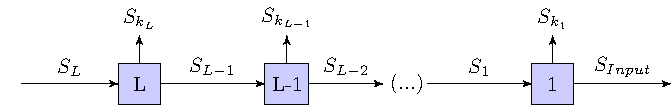
\includegraphics{Figures/chapter_interpretation/figures/score_map.pdf}
	\caption{Score distribution through layers}
	\label{score:fig:score_map}
\end{figure}

The output score is expressed as:

\begin{equation}
S_L = \sum_{l=1}^L \left ( \sum S_{k_l} \right ) + \left ( \sum S_{Input} \right )
\end{equation}

being $S_L$ last layer feature score, $S_{k_l}$ the constant tensors of each layer, $\sum S_{k_l}$ the element-wise sum of scores and $\sum S_{k_l}$ the pixel-wise sum of scores.

Second, if required, $S_{k_l}$ values obtained from each of the layers can also be mapped into the input space using an additional final procedure described in section \ref{score:sec:mapping-input}.

Receptive field pixel maps allow the identification of the parts of the image that the network is considering important. In our case study, DR classification, it is not only important to detect the pixel-size micro lesions but also the clusters of lesions localized in different parts of the image. Taking into account each receptive field contributions apart from the input, facilitates the detection of such clusters and not only the individual contributions of each pixel. 

Now, we explain the propagation process for different components of the DL classifier.

\subsection{Score propagation through an activation function node} 

In fig. \ref{score:fig:score_af} we show the activation function node. A input activation $a_i$ is transformed into the output activation as $a_o = \phi(a_i)$. Taking $S_o = \lambda_o a_o$ and substituting $a_o$, we get $S_o = \lambda_o \phi(a_i)$. According to proposition 1, we have also that $S_i = \lambda_i a_i$. For ReLU family functions ($\phi(x) = max(0, kx)$), $S_i$ continues verifying the proposition. For other type of activation functions, as we are calculating the score of a particular image, we can consider the network to have parameter-wise activation functions. For a particular image, we can consider the first order Taylor expansion and see the activation function as a linear function of the form $\phi(a_i) = [\phi(a^*_i) + \phi'(a^*_i)(a_i - a^*_i)]$, where $a^*_i$ is a value close enough to $a_i$ to have a good approximation of $\phi$. After this transformation, the proposition holds for every type of activation function. Substituting and reordering the expression of $S_o$ we obtain that:

\begin{equation}
S_o = \lambda_o[\phi(a^*_i) - \phi'(a^*_i)a^*_i] + \lambda_o \phi'(a^*_i)a_i
\end{equation}

Now, the output score can be split in two parts: a constant one that is independent of the activation and belongs to the node and another one dependent on the activation. For ReLU, they are $S_o = S_i$ and $S_k = 0$.

\begin{figure}[!ht]
	\centering
	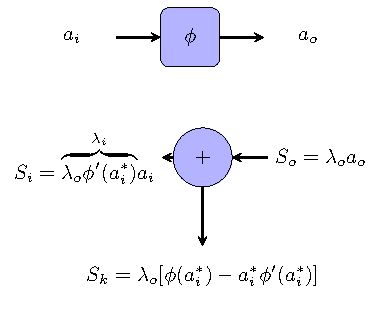
\includegraphics{Figures/chapter_interpretation/figures/score_af.pdf}
	\caption{Score propagation through an activation function node}
	\label{score:fig:score_af}
\end{figure}

\subsection{Score propagation through a batch normalization node} 

The function implemented in a batch normalization node is $a_o = \beta + \gamma (\frac{a_i - \mu}{\sigma})$. Having $S_o = \lambda_o a_o$, $S_o$ is also $S_o = \lambda_o ( \beta + \gamma (\frac{a_i - \mu}{\sigma}))$. Reordering the expression, we can separate the input independent constants: 

\begin{equation}
S_o = \lambda_o (\beta - \gamma \frac{\mu}{\sigma}) + \lambda_o \frac{\gamma}{\sigma}a_i
\end{equation}

As we see, the output score can be exactly split into a constant value $S_k = \lambda_o (\beta - \gamma \frac{\mu}{\sigma})$ that is a inherent property of the node and is completely independent of $a_i$ and into $S_i = (\lambda_o \frac{\gamma}{\sigma})a_i = \lambda_i S_i$ following Proposition 2, being $\lambda_i = \lambda_o \frac{\gamma}{\sigma}$ (see fig. \ref{score:fig:score_bn})

\begin{figure}[!ht]
	\centering
	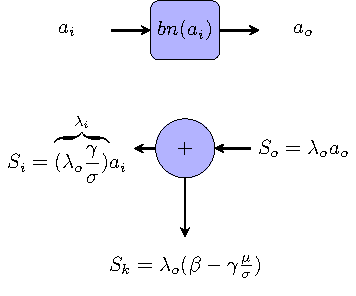
\includegraphics{Figures/chapter_interpretation/figures/score_bn.pdf}
	\caption{Score propagation through an batch normalization node}
	\label{score:fig:score_bn}
\end{figure}

\subsection{Score propagation through a convolutional layer}

In the forward propagation of a two dimensional convolution of an image, the set of all the different feature activations of a predefined locality are linearly combined to get the output $a_o$ (see fig. \ref{score:fig:convolution_score}). Backpropagating a score in a convolutional layer requires to divide it into all its individual components. Every component can be either positive or negative. There is also a bias part that comes from the inherent nature of the layer and that is not attributable to any of the inputs and that must be treated also as a property of the layer. Due to the nature of the convolution operator, every input node contributes to the calculation of different outputs. This is the reason why every input receives a contribution of the score of the different outputs that are, then, summed up.

\begin{figure}[!ht]
	\centering
	\begin{subfigure}{0.4\textwidth}
		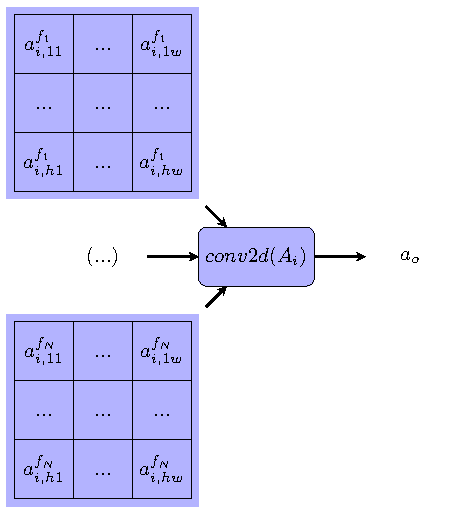
\includegraphics[scale=0.5]{Figures/chapter_interpretation/figures/score_conv2d.pdf}
	\end{subfigure}
	~ % spacing  ~, \quad, \qquad
	\begin{subfigure}{0.4\textwidth}
		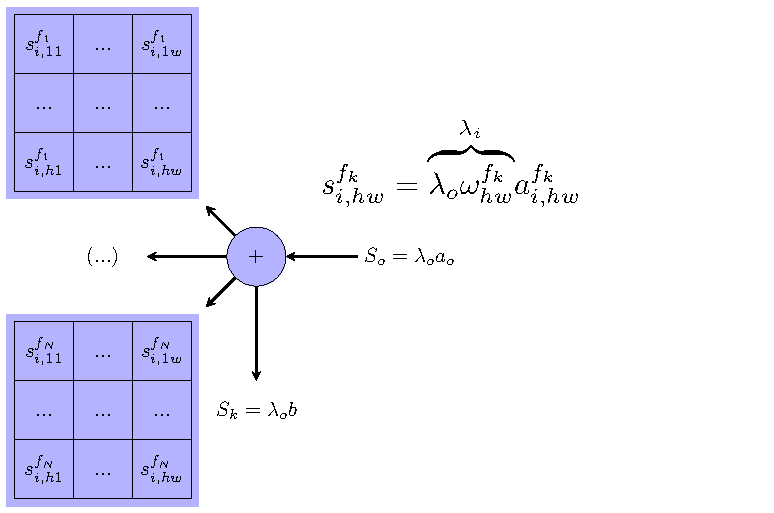
\includegraphics[scale=0.5]{Figures/chapter_interpretation/figures/score_conv2d_score.pdf}
	\end{subfigure}
	\caption[Convolution score calculation]{Convolution score calculation. Score spreads into the different inputs. The bias related part of the score is not backpropagated.}
	\label{score:fig:convolution_score}
\end{figure}


\subsection{Score propagation through pooling layers}

The score propagation through a max-pooling layer is straightforward. The score of output is copied into the input that was selected in the forward pass (see fig. \ref{score:fig:score_pooling}). For average pooling, it is also straightforward. The score value is split into $N$ equal parts, being $N$ the number of inputs (see fig. \ref{score:fig:score_pooling}).

\begin{figure}[!ht]
	\centering
	\begin{subfigure}{0.4\textwidth}
		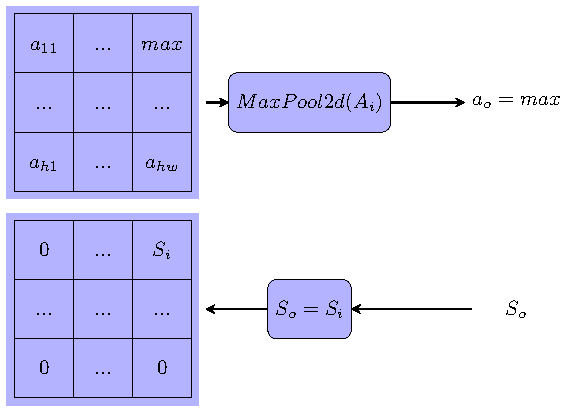
\includegraphics[scale=0.5]{Figures/chapter_interpretation/figures/score_maxpool.pdf}
		\caption{Max-Pooling}
	\end{subfigure}
	~ % spacing  ~, \quad, \qquad
	\begin{subfigure}{0.4\textwidth}
		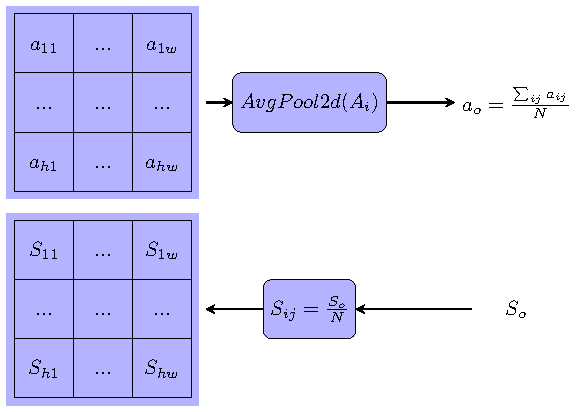
\includegraphics[scale=0.5]{Figures/chapter_interpretation/figures/score_avgpool.pdf}
		\caption{Avg-Pooling}
	\end{subfigure}
	\caption{Score propagation through different pooling layers}
	\label{score:fig:score_pooling}
\end{figure}

\subsection{Score propagation through a fully connected layer} 

A fully connected layer is a linear combination of the input activations and their weights. The final score is split into the individual elements, leaving apart the bias that becomes the constant score contribution of the own layer (see fig. \ref{score:fig:score_fc}).

\begin{figure}[!ht]
	\centering
	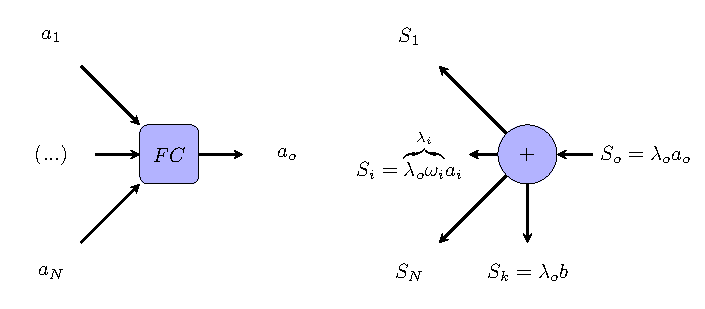
\includegraphics{Figures/chapter_interpretation/figures/score_fc.pdf}
	\caption{Score propagation through a fully connected node}
	\label{score:fig:score_fc}
\end{figure}

\subsection{Score propagation through a dropout layer}

Dropout in evaluation time weights the output to a value proportional to the dropout probability: $a_o = (1-d)a_i$. Inserting this equation into $S_o = \lambda_o a_o$ and applying the score conservation through the node ($S_o = S_i$ in this case, due to the absence of constant score), we get that the final equation:

\begin{equation}
\lambda_i = \lambda_o (1-d)
\end{equation}

\begin{figure}[!ht]
	\centering
	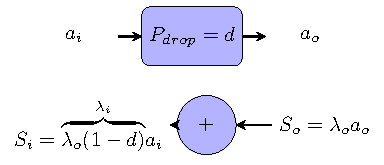
\includegraphics{Figures/chapter_interpretation/figures/score_dropout.pdf}
	\caption{Score propagation through a dropout node}
	\label{score:fig:score_dropout}
\end{figure}

\subsection{Mapping the score of hidden layers and $S_k$ into input-space} \label{score:sec:mapping-input}

We know that every node has two score constituents: one input-dependent, that can be easily forwarded, and another one RF-dependent, i.e layer-dependent. At this point, we are going to describe a method to transport backwards also such last values into the input-space. From \citep{luo2016understanding}, we know that the effective RF is not equal to the theoretical RF. The effective one acts more like a 2D-gaussian function, where the points located in the borders contribute less than the center ones. Using such prior information, it is possible to make an approximate conversion of the full and constant scores in the hidden-space to the input-space using a 2D-gaussian prior. For example, for a 20x20 hidden layer with a RF of 189x189 pixels, we know that each one of such points is a representation value of a 189x189 RF in the input-space. Having a prior information about the statistical distribution of the input-space pixels (in this case gaussian), it is possible to go back. Summing up 20x20 gaussian distributions of mean equal to the hidden-space values and summing up the coincident points, it is possible to map the distribution into input-space. We fixed $RF = 2\sigma$ as an approximate distribution of the scores that seems acceptable \citep{luo2016understanding}, since 98\% of the information of the gaussian is inside the RF. We normalize the function to fit 100\% of the information inside the RF.

%\section{Classification Model for Diabetic Retinoathy}\label{score:sec:class}

\section{Results}\label{score:sec:results}

The classifier used for application of the interpretation model is the one described in chapter \ref{Chapter:Classification}. In figure \ref{class2:fig:drmodel} can be found the model architecture.

\subsection{Pixel and receptive field map generation}

In this subsection we describe the steps followed in the score calculation of a test set sample. Fig. \ref{score:fig:retine_test} is tagged in the test set as class 4. For this image the model reports the next classification scores (previous to soft-max): $C_0 = -451.2$, $C_1 = -229.0$, $C_2 = -53.4$, $C_3 = +37.4$ and $C_4 = +73.2$. Being $C_4$ the highest value, the image is correctly classified as class 4. In fig. \ref{score:fig:retine_sample_score_map} we show a black and white version of the image with the distribution of the positive contributions to the class 4 total score in input space. Having the total score map is possible to visualize different versions of it, showing the negative contributions, or the most positive ones, or defining a positive threshold for displaying only the higher scores. In this way is possible to identify the points that contribute the most to a particular classification. There should be a correlation between such points and lesions in the eye if we are studying, as in this sample, a severe disease class.

\begin{figure}[ht]
	\centering
	\begin{subfigure}{0.4\textwidth}
		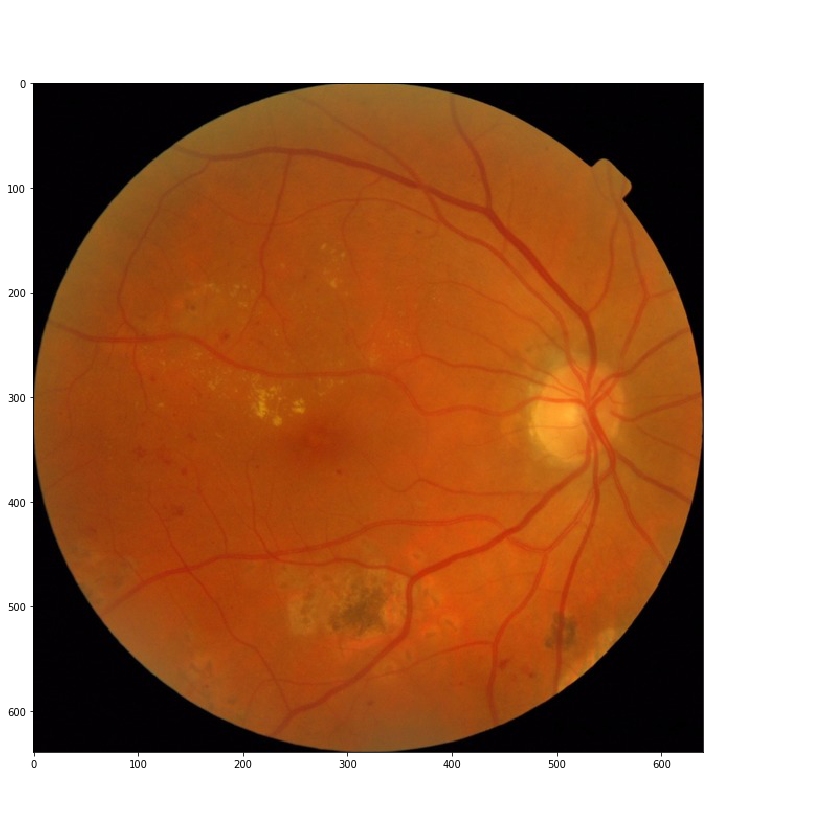
\includegraphics[width=\textwidth]{Figures/chapter_interpretation/figures/maps/retina.png}
		\caption{Network input image}
		\label{score:fig:retine_sample}
	\end{subfigure}
	~ % spacing  ~, \quad, \qquad
	\begin{subfigure}{0.4\textwidth}
		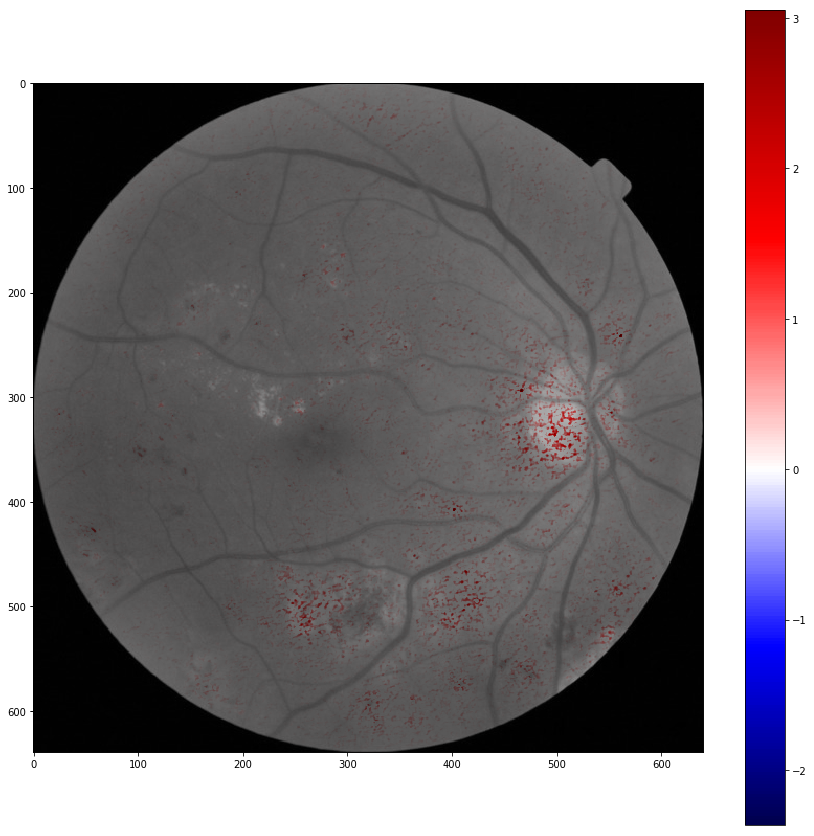
\includegraphics[width=\textwidth]{Figures/chapter_interpretation/figures/maps/inputc.png}
		\caption{Class 4 positive score map}
		\label{score:fig:retine_sample_score_map}
	\end{subfigure}\\
	\caption{Class 4 sample image}	
	\label{score:fig:retine_test}
\end{figure}

Figure \ref{score:fig:scoremaps2} show the aggregated scores for different intermediate layers. For visualization purposes, layer scores are presented considering the layer as a unique block combination of \emph{convolution - batch normalization - ReLU}. The output of this function block can be mathematically expressed as $O = max(0, \beta + \gamma(\frac{WI + b - \mu}{sigma})$, being $S_O = \lambda (\beta + \gamma \frac{b - \mu}{\sigma}) + \lambda \frac{\gamma}{\sigma}WI$. In this way $S_I = \lambda \frac{\gamma}{\sigma}WI$ and $S_k = \lambda (\beta + \gamma \frac{b - \mu}{\sigma})$. 

\begin{figure}[!ht]
	\centering
	\begin{subfigure}{0.4\textwidth}
		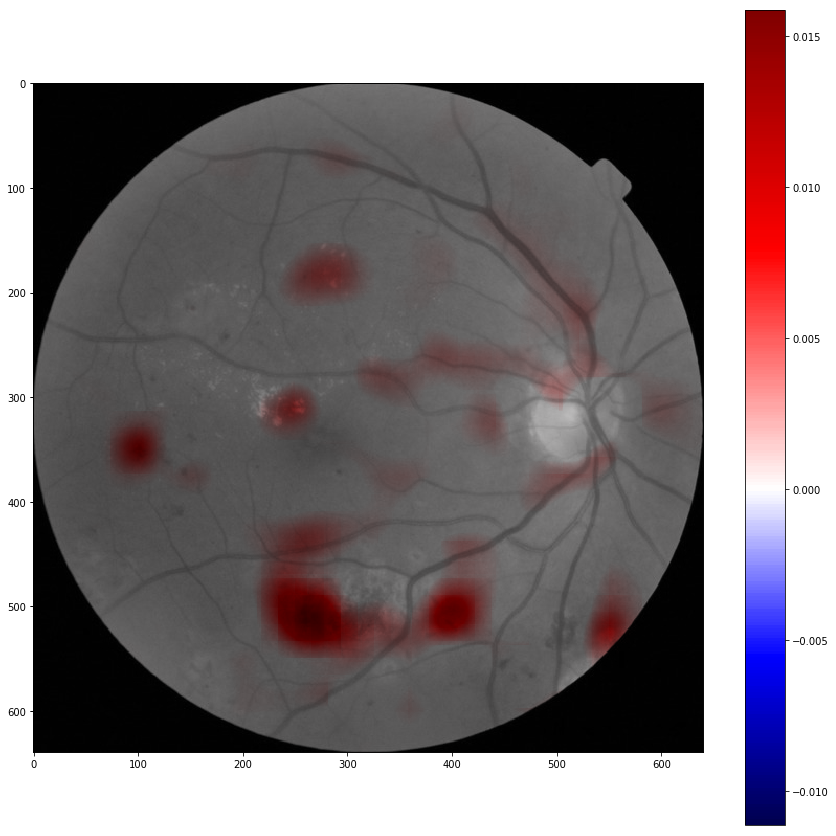
\includegraphics[width=\textwidth]{Figures/chapter_interpretation/figures/maps/rf61c.png}
		\caption{Layer 8 (RF=61x61)}
		\label{score:fig:score_rf61}
	\end{subfigure}
	~ % spacing  ~, \quad, \qquad
	\begin{subfigure}{0.4\textwidth}
		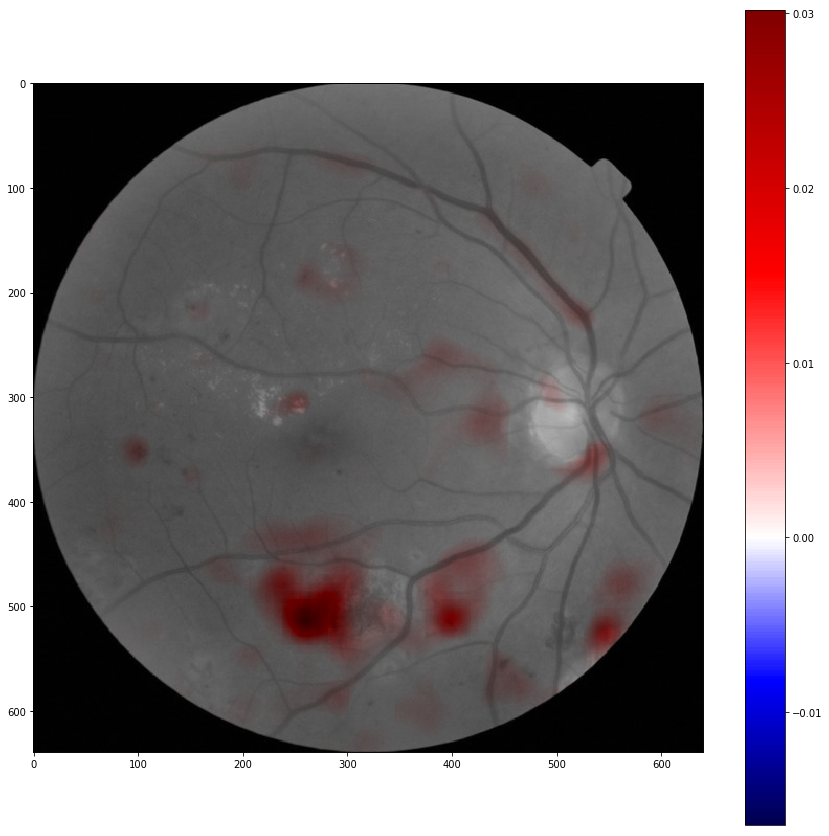
\includegraphics[width=\textwidth]{Figures/chapter_interpretation/figures/maps/rf45c.png}
		\caption{Layer 7 (RF=45x45)}
		\label{score:fig:score_rf45}
	\end{subfigure}\\
	\begin{subfigure}{0.4\textwidth}
		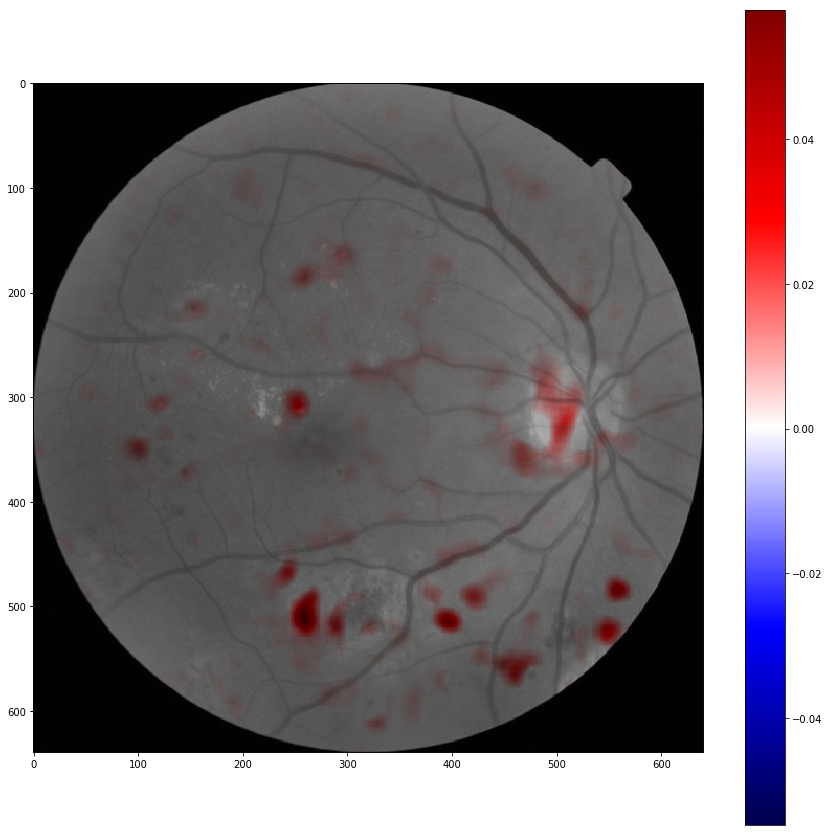
\includegraphics[width=\textwidth]{Figures/chapter_interpretation/figures/maps/rf29c.png}
		\caption{Layer 6 (RF=29x29)}
		\label{score:fig:score_rf29}
	\end{subfigure}
	~ % spacing  ~, \quad, \qquad
	\begin{subfigure}{0.4\textwidth}
		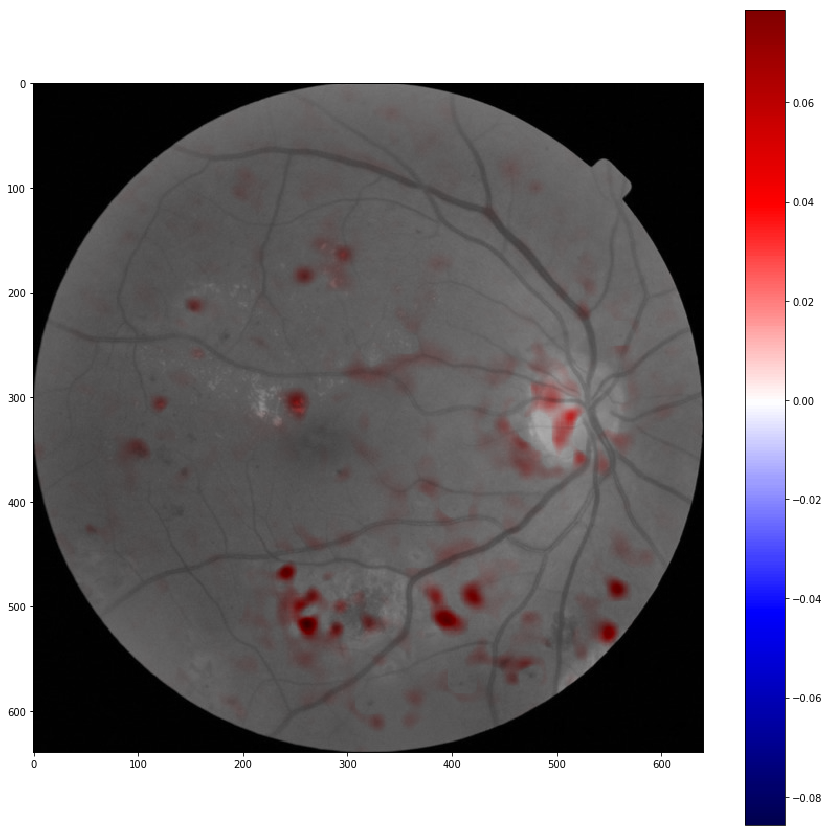
\includegraphics[width=\textwidth]{Figures/chapter_interpretation/figures/maps/rf21c.png}
		\caption{Layer 5 (RF=21x21)}
		\label{score:fig:score_rf21}
	\end{subfigure}\\
	\caption[Class 4 sample intermediate score maps]{Some of the class 4 intermediate score maps generated for the sample image}
	\label{score:fig:scoremaps2}
\end{figure}

%Fig. \ref{score:fig:feature_scores} shows layer 16 individual feature score distribution for the class 4. 

%\begin{figure}[!ht]
%	\centering
%	\includegraphics[width=\textwidth]{./chapter_interpretation/figures/maps/f4.png}
%	\caption{Sample image layer 16 class 4 feature scores}
%	\label{score:fig:feature_scores}
%\end{figure}

Individual feature scores are first calculated, \emph{receptive field-wise} summed up and mapped into input-space (section \ref{score:sec:mapping-input}). The same is done for $S_k^{(l)} \quad \forall l \in L$. Score inputs can be combined with constant scores to define a unique input score map. The sum of these scores is equal to the last layer inference score and determines the relative importance of every pixel in the final decision. A density plot and a standard deviation can also be calculated. In order to determine the importance of pixels, as noted before, it is possible to restrict the visualization to positive scores or also be even more restrictive and visualize only pixels with a score greater than a predefined threshold, for example $n \sigma$. These score maps are useful for interpreting the reasons behind a classification, for detecting the cause of non-expected classifications, for example pixels with excessive importance in the final decision, conclusions based only on partial or incorrect information, etc. 

%\vspace{1cm} % just to get a page break. Remove if not required
In red in figure \ref{score:fig:scoremaps2} we have the zones that are contributing positively to classify the image as class 4. It is possible to plot also the zones contributing negatively to the classification. In case of being analyzing a class 4, negative score zones(not shown) would be zones without lesions. For clarity purposes only positive values are shown. Regions of red and blue pixels are sequentially fine-grained as the size of the receptive field decreases. Having the possibility to choose the RF size, permits to analyze the areas contributing to image classification at different levels of precision.

Intermediate scores are also very useful for identifying clusters of micro-lesions and evaluate its combined weight in the final score. They enable the location of lesion clusters and also zones not affected by the disease. For example, in layer 12, with a receptive field of 253x253 the network identifies two zones with high contribution to class 4 score. In layer 11, where the receptive field is smaller (189x189) we see how the detail is increasing, showing more localized zones. In layer 8, 7, 6, 5 and finally input show increasing level of detail dividing big clusters into smaller ones until reaching the input space where individual pixels are identified.

\begin{figure}[!ht]
	\centering
	\begin{subfigure}{0.45\textwidth}
		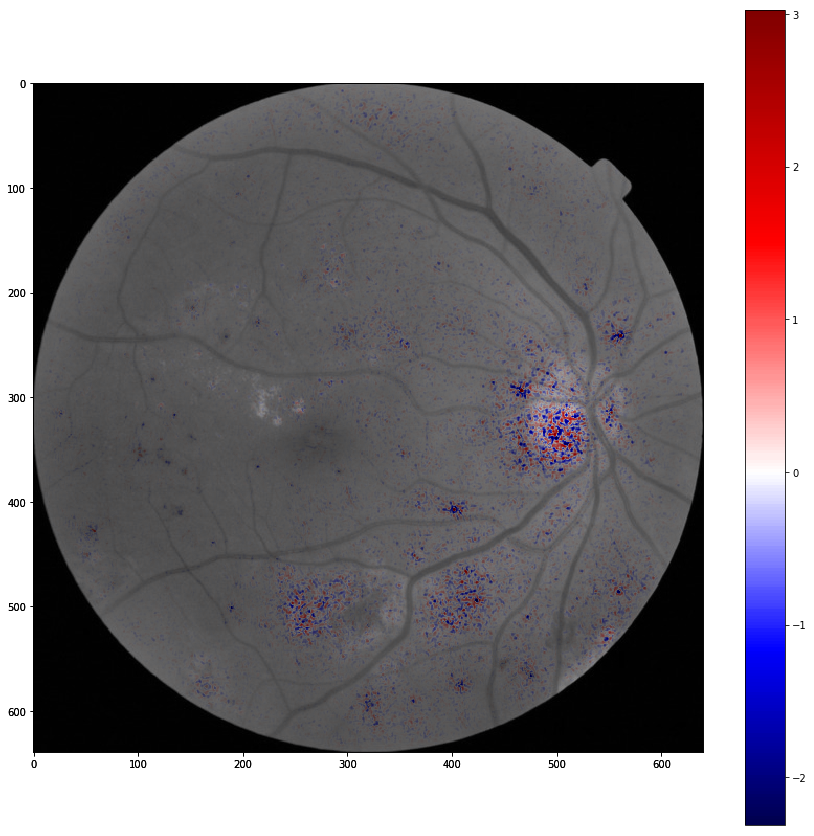
\includegraphics[width=\textwidth]{Figures/chapter_interpretation/figures/maps/inp.png}
		\caption{$S_I$}
		\label{score:fig:score_input}
	\end{subfigure}
	~ % spacing  ~, \quad, \qquad
	\begin{subfigure}{0.45\textwidth}
		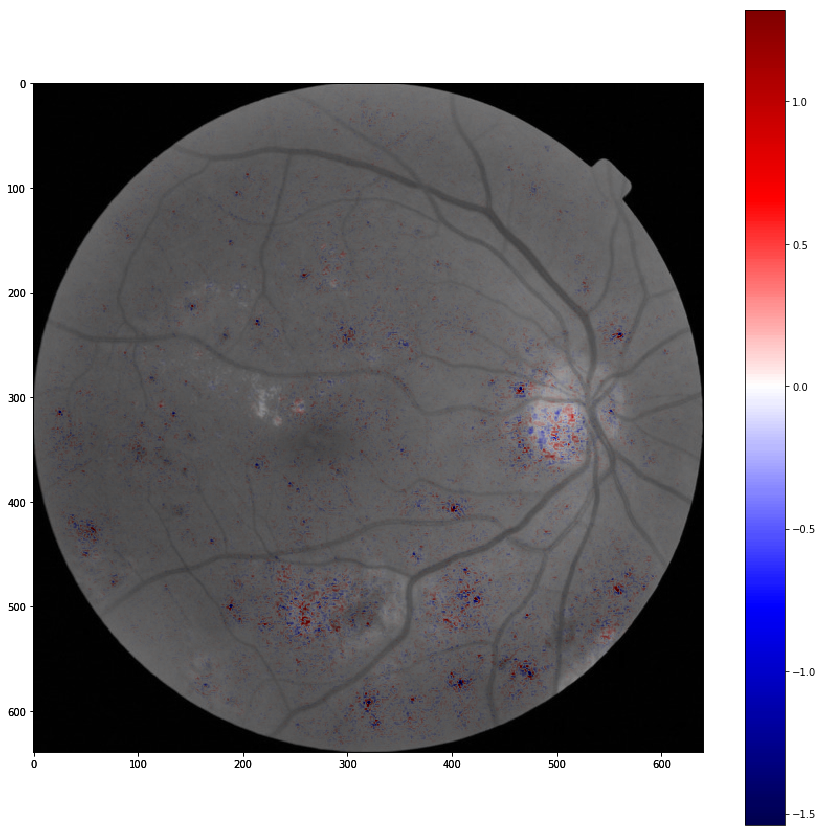
\includegraphics[width=\textwidth]{Figures/chapter_interpretation/figures/maps/kmap.png}
		\caption{$\sum_{l=1}^L S_{k_l}$}
		\label{score:fig:score_kmapped}
	\end{subfigure}
	~ % spacing  ~, \quad, \qquad
	\begin{subfigure}{0.45\textwidth}
		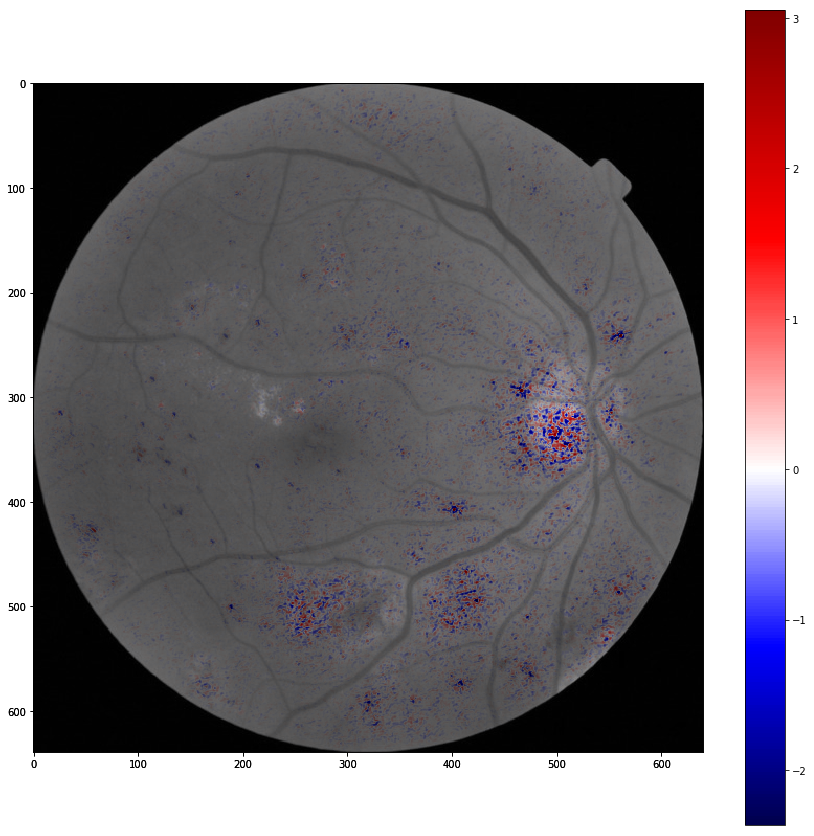
\includegraphics[width=\textwidth]{Figures/chapter_interpretation/figures/maps/tot.png}
		\caption{$S_{T}$}
		\label{score:fig:score_total}
	\end{subfigure}
	\caption[Total score maps]{Total score maps: $S_{T} = S_I + \sum_{l=1}^L S_{k_l}$}
	\label{score:fig:total_score_maps}
\end{figure}


\begin{table}[ht]
	\centering
	\begin{tabular}{c c c c c c c}
		\hline
		\hline                        
		Map & $\mu$ & $\sigma$ & Max & Min & Sum & Non-null \\ 
		\hline
		$S_I$ & 0.0 & 0.17 & +19.6 & -9.1 & +6.7 & 99.97\%  \\
		$\sum S_k$ & 0.0 & 0.06 & +2.7 & -3.7 & +66.5 & 99.90\% \\
		$S_T$ & 0.0 & 0.19 & +20.2 & -9.6 & +73.2 & 99.97\% \\  
		\hline
	\end{tabular}
	\caption{Class 4 score map statistics for the analyzed image}
	\label{score:table:score_stats}
\end{table}

Finally, in figure \ref{score:fig:total_score_maps} we present the total score map for the analyzed image, plotting not only pixels with positive contribution (red) but also the negative ones (blue). The score input $S_I$ (fig. \ref{score:fig:score_input}) represents the map obtained from back-propagating the part that linearly depends on inputs. The score constant $\sum S_k$ (fig. \ref{score:fig:score_kmapped}) is the map obtained from summing up $S_k$ for all layers mapped into input space. Score total $S_T$ (fig. \ref{score:fig:score_total}) is the sum of the two previous maps and represent the total class 4 score distribution. The sum of all the scores of the pixels is equal to the output score. Table \ref{score:table:score_stats} shows some statistics of the three score maps. We can see that $\sum S_k$ is the score map contributing the most to final total score. This map is flatter than $S_I$, so qualitatively $S_I$ and $S_T$ are very similar. It seems that $\sum S_k$ acts more as a mild shifting of each receptive field considered by the network and $S_I$ acts reinforcing the importance of representative individual pixels.

\section{Conclusions}\label{score:sec:conclusions}

In this chapter we proposed a method for generating, for every class, score importance pixel maps, providing ophthalmologists the possibility of both inference and interpretation. The reduced number of model parameters enables the use of these algorithms even in low resources devices, like mobile phones. The score generation is done back-propagating layer-wise only the score part that depends on the inputs and leaving the constant part as a contribution to the score of the considered layer. In this way, this method is are able to generate scores in a unique and exact way. 

Additionally, we have developed a technique, consisting on applying a 2D-gaussian prior over the RFs, for mapping the constant hidden-space scores to the input. With this technique we can generate a unique score map representative of the class, making possible to distribute the 100\% score class information of the output layer. 

We concluded also that for a good understanding of the causes behind a classification, not only the pixel-space maps should be considered, but also the intermediate ones. The combination of the micro-information given by the input space maps with the macro-information obtained from intermediate scores is the key for understanding the results and to help the medical personnel to improve the diagnosis processes.

